%%%%%%%%%%%%%%%%%%%%%%%%%%%%%%%%%%%%%%%%%
% University Assignment Title Page 
% LaTeX Template
% Version 1.0 (27/12/12)
%
% This template has been downloaded from:
% http://www.LaTeXTemplates.com
%
% Original author:
% WikiBooks (http://en.wikibooks.org/wiki/LaTeX/Title_Creation)
%
% License:
% CC BY-NC-SA 3.0 (http://creativecommons.org/licenses/by-nc-sa/3.0/)
% 
% Instructions for using this template:
% This title page is capable of being compiled as is. This is not useful for 
% including it in another document. To do this, you have two options: 
%
% 1) Copy/paste everything between \begin{document} and \end{document} 
% starting at \begin{titlepage} and paste this into another LaTeX file where you 
% want your title page.
% OR
% 2) Remove everything outside the \begin{titlepage} and \end{titlepage} and 
% move this file to the same directory as the LaTeX file you wish to add it to. 
% Then add %%%%%%%%%%%%%%%%%%%%%%%%%%%%%%%%%%%%%%%%%
% University Assignment Title Page 
% LaTeX Template
% Version 1.0 (27/12/12)
%
% This template has been downloaded from:
% http://www.LaTeXTemplates.com
%
% Original author:
% WikiBooks (http://en.wikibooks.org/wiki/LaTeX/Title_Creation)
%
% License:
% CC BY-NC-SA 3.0 (http://creativecommons.org/licenses/by-nc-sa/3.0/)
% 
% Instructions for using this template:
% This title page is capable of being compiled as is. This is not useful for 
% including it in another document. To do this, you have two options: 
%
% 1) Copy/paste everything between \begin{document} and \end{document} 
% starting at \begin{titlepage} and paste this into another LaTeX file where you 
% want your title page.
% OR
% 2) Remove everything outside the \begin{titlepage} and \end{titlepage} and 
% move this file to the same directory as the LaTeX file you wish to add it to. 
% Then add %%%%%%%%%%%%%%%%%%%%%%%%%%%%%%%%%%%%%%%%%
% University Assignment Title Page 
% LaTeX Template
% Version 1.0 (27/12/12)
%
% This template has been downloaded from:
% http://www.LaTeXTemplates.com
%
% Original author:
% WikiBooks (http://en.wikibooks.org/wiki/LaTeX/Title_Creation)
%
% License:
% CC BY-NC-SA 3.0 (http://creativecommons.org/licenses/by-nc-sa/3.0/)
% 
% Instructions for using this template:
% This title page is capable of being compiled as is. This is not useful for 
% including it in another document. To do this, you have two options: 
%
% 1) Copy/paste everything between \begin{document} and \end{document} 
% starting at \begin{titlepage} and paste this into another LaTeX file where you 
% want your title page.
% OR
% 2) Remove everything outside the \begin{titlepage} and \end{titlepage} and 
% move this file to the same directory as the LaTeX file you wish to add it to. 
% Then add %%%%%%%%%%%%%%%%%%%%%%%%%%%%%%%%%%%%%%%%%
% University Assignment Title Page 
% LaTeX Template
% Version 1.0 (27/12/12)
%
% This template has been downloaded from:
% http://www.LaTeXTemplates.com
%
% Original author:
% WikiBooks (http://en.wikibooks.org/wiki/LaTeX/Title_Creation)
%
% License:
% CC BY-NC-SA 3.0 (http://creativecommons.org/licenses/by-nc-sa/3.0/)
% 
% Instructions for using this template:
% This title page is capable of being compiled as is. This is not useful for 
% including it in another document. To do this, you have two options: 
%
% 1) Copy/paste everything between \begin{document} and \end{document} 
% starting at \begin{titlepage} and paste this into another LaTeX file where you 
% want your title page.
% OR
% 2) Remove everything outside the \begin{titlepage} and \end{titlepage} and 
% move this file to the same directory as the LaTeX file you wish to add it to. 
% Then add \input{./title_page_1.tex} to your LaTeX file where you want your
% title page.
%
%%%%%%%%%%%%%%%%%%%%%%%%%%%%%%%%%%%%%%%%%
%\title{Title page with logo}
%----------------------------------------------------------------------------------------
%	PACKAGES AND OTHER DOCUMENT CONFIGURATIONS
%----------------------------------------------------------------------------------------

\documentclass[12pt]{article}
\usepackage[english]{babel}
%\usepackage[utf8x]{inputenc}
\usepackage[utf8]{inputenc}
\usepackage{amsmath}
\usepackage{graphicx}
\usepackage[colorinlistoftodos]{todonotes}
\usepackage{pdfpages}
\usepackage[
backend=biber,
style=numeric,
sorting=none
]{biblatex}

\addbibresource{sample.bib} %Imports bibliography file

\title{Bibliography management: \texttt{biblatex} package}
\author{Share\LaTeX}
\date{ }


\begin{document}

\begin{titlepage}

\newcommand{\HRule}{\rule{\linewidth}{0.5mm}} % Defines a new command for the horizontal lines, change thickness here

\center % Center everything on the page
 
%----------------------------------------------------------------------------------------
%	HEADING SECTIONS
%----------------------------------------------------------------------------------------

\textsc{\LARGE Sint-Jan-Berchmanscollege Brussel}\\[1.5cm] % Name of your university/college
\textsc{\Large Economie Wiskunde 6}\\[0.5cm] % Major heading such as course name
\textsc{\large Nederlands}\\[0.5cm] % Minor heading such as course title

%----------------------------------------------------------------------------------------
%	TITLE SECTION
%----------------------------------------------------------------------------------------

\HRule \\[0.4cm]
{ \huge \bfseries Leesportfolio}\\[0.4cm] % Title of your document
\HRule \\[1.5cm]
 
%----------------------------------------------------------------------------------------
%	AUTHOR SECTION
%----------------------------------------------------------------------------------------

\begin{minipage}{0.4\textwidth}
\begin{flushleft} \large
\emph{Leerling:}\\
Benoît \textsc{Stroobants} % Your name
\end{flushleft}
\end{minipage}
~
\begin{minipage}{0.4\textwidth}
\begin{flushright} \large
\emph{Leerkracht:} \\
Mr R. \textsc{Vandeweerdt} % Supervisor's Name
\end{flushright}
\end{minipage}\\[2cm]

% If you don't want a supervisor, uncomment the two lines below and remove the section above
%\Large \emph{Author:}\\
%John \textsc{Smith}\\[3cm] % Your name

%----------------------------------------------------------------------------------------
%	DATE SECTION
%----------------------------------------------------------------------------------------

{\large \today}\\[2cm] % Date, change the \today to a set date if you want to be precise

%----------------------------------------------------------------------------------------
%	LOGO SECTION
%----------------------------------------------------------------------------------------


\includegraphics[width=0.3\textwidth]{Foto's/Sint_Jan_Berchmanscollege_logo2.png}\\ % Include a department/university logo - this will require the graphicx package

 
%----------------------------------------------------------------------------------------

\vfill % Fill the rest of the page with whitespace

\end{titlepage}


\renewcommand*\contentsname{Inhoudstafel}

\tableofcontents
\newpage
\vspace*{\fill}
\begin{center}
\addcontentsline{toc}{section}{Opdracht 1: Ervaringsverslag}
\newcommand{\HRule}{\rule{\linewidth}{0.5mm}}
\HRule \\[0.4cm]
\section*{Opdracht 1: Ervaringsverslag \cite{1}}
\HRule \\[1.5cm]
\end{center}
\vspace*{\fill}
   
\includepdf[page=-]{Opdracht 1.pdf}
       

\newpage
\vspace*{\fill}
\begin{center}
\addcontentsline{toc}{section}{Opdracht 2: Structureel-analytisch verslag van een kortverhaal}
\newcommand{\HRule}{\rule{\linewidth}{0.5mm}}
\HRule \\[0.4cm]
\section*{Opdracht 2: Structureel-analytisch verslag van een kortverhaal \cite{2}}
\HRule \\[1.5cm]
\end{center}
\vspace*{\fill}
   
%\includepdf[page=-]{Opdracht 2.pdf}

\newpage
\vspace*{\fill}
\begin{center}
\addcontentsline{toc}{section}{Opdracht 3: Creatieve opdracht}
\newcommand{\HRule}{\rule{\linewidth}{0.5mm}}
\HRule \\[0.4cm]
\section*{Opdracht 3: Creatieve opdracht \cite{3}}
\HRule \\[1.5cm]
\end{center}
\vspace*{\fill}
   
%\includepdf[page=-]{Opdracht 3.pdf}

\newpage
\vspace*{\fill}
\begin{center}
\addcontentsline{toc}{section}{Opdracht 4: Mediagerichte opdracht}
\newcommand{\HRule}{\rule{\linewidth}{0.5mm}}
\HRule \\[0.4cm]
\section*{Opdracht 4: Mediagerichte opdracht \cite{4}}
\HRule \\[1.5cm]
\end{center}
\vspace*{\fill}
   
%
\includepdf[page=-]{Opdracht 4.pdf}

\newpage
\vspace*{\fill}
\begin{center}
\addcontentsline{toc}{section}{Opdracht 5: Een theaterverslag}
\newcommand{\HRule}{\rule{\linewidth}{0.5mm}}
\HRule \\[0.4cm]
\section*{Opdracht 5: Een theaterverslag \cite{5}}
\HRule \\[1.5cm]
\end{center}
\vspace*{\fill}
   
%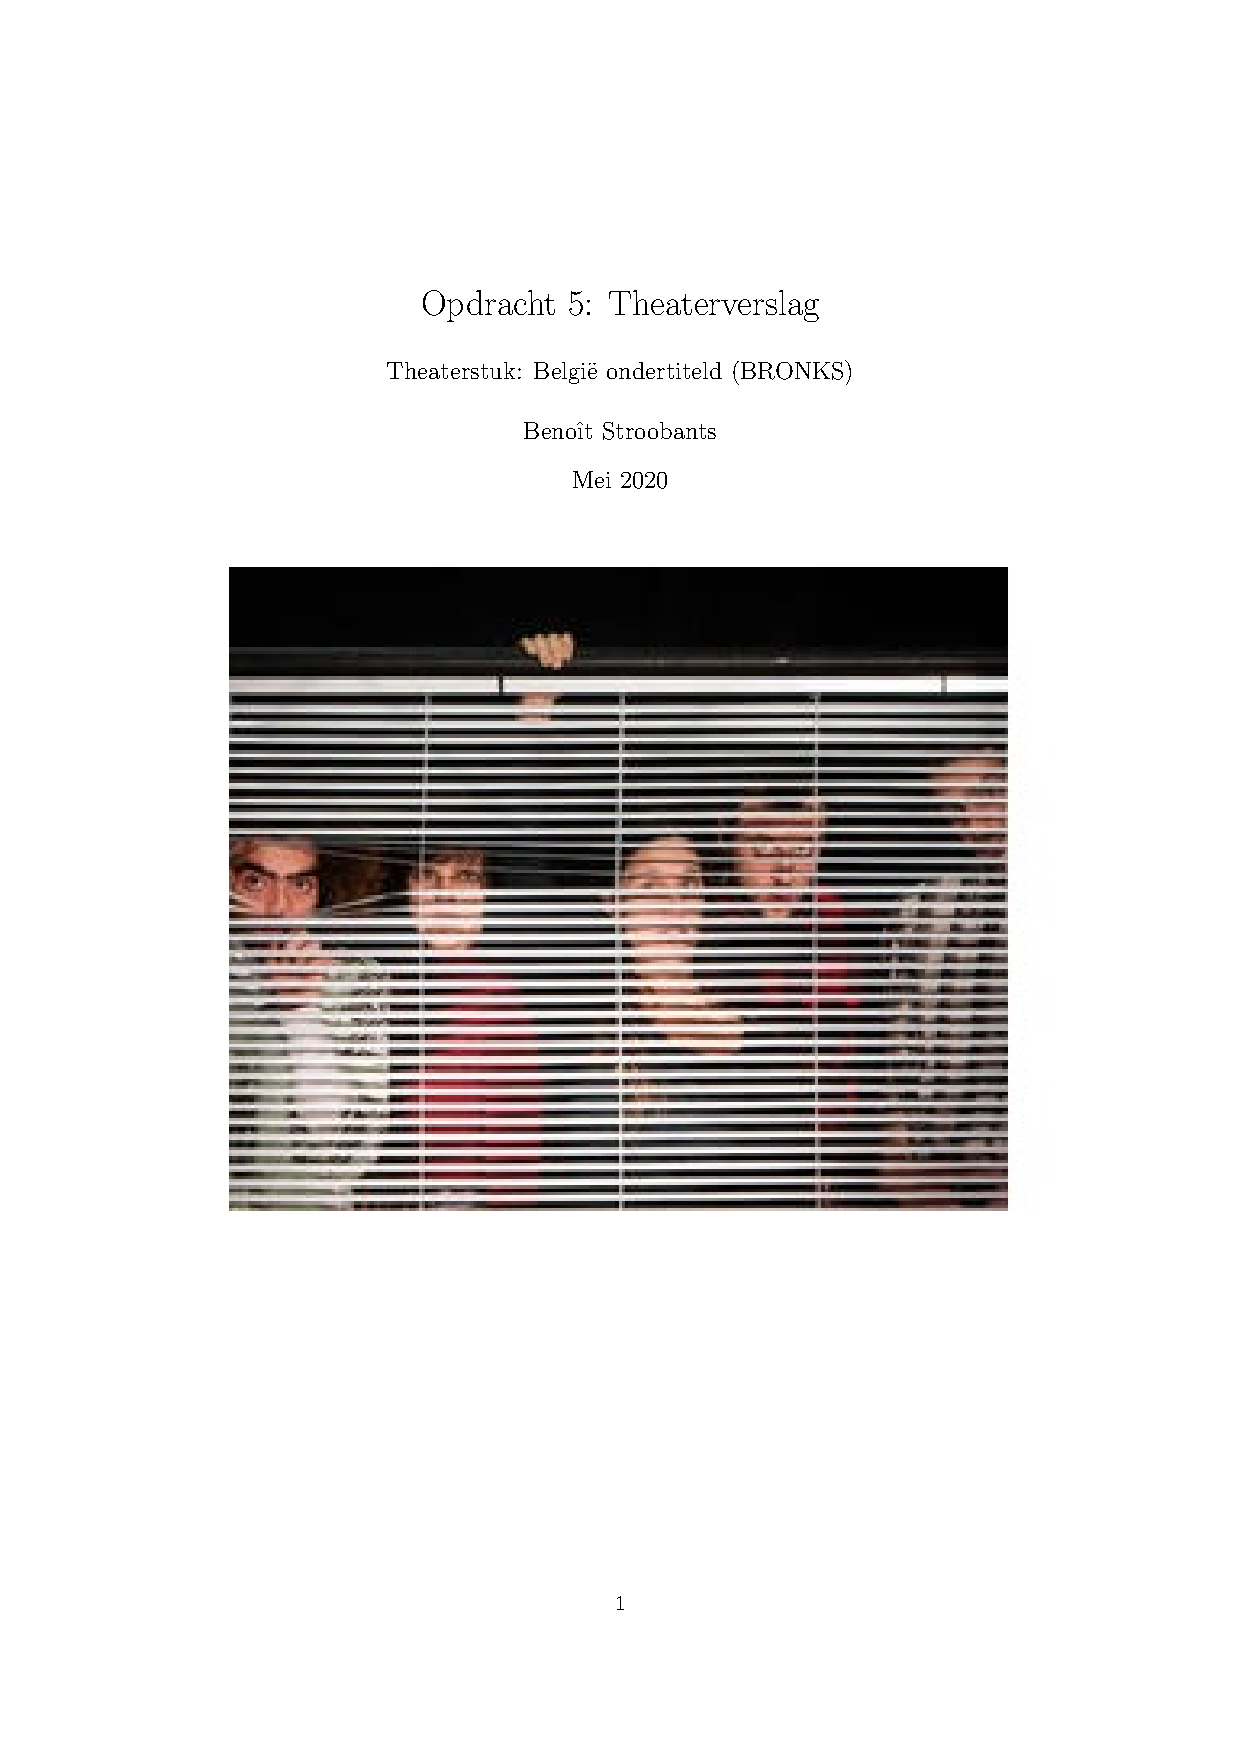
\includepdf[page=-]{Opdracht 5.pdf}

\newpage
\vspace*{\fill}
\begin{center}
\addcontentsline{toc}{section}{Opdracht 6: Een balansverslag}
\newcommand{\HRule}{\rule{\linewidth}{0.5mm}}
\HRule \\[0.4cm]
\section*{Opdracht 6: Een balansverslag}
\HRule \\[1.5cm]
\end{center}
\vspace*{\fill}
   
%\includepdf[page=-]{Opdracht 6.pdf}

\newpage


\printbibliography[heading=bibintoc,title={Bibliografie}] %Prints the entire bibliography with the titel "Whole bibliography"
         
\end{document} to your LaTeX file where you want your
% title page.
%
%%%%%%%%%%%%%%%%%%%%%%%%%%%%%%%%%%%%%%%%%
%\title{Title page with logo}
%----------------------------------------------------------------------------------------
%	PACKAGES AND OTHER DOCUMENT CONFIGURATIONS
%----------------------------------------------------------------------------------------

\documentclass[12pt]{article}
\usepackage[english]{babel}
%\usepackage[utf8x]{inputenc}
\usepackage[utf8]{inputenc}
\usepackage{amsmath}
\usepackage{graphicx}
\usepackage[colorinlistoftodos]{todonotes}
\usepackage{pdfpages}
\usepackage[
backend=biber,
style=numeric,
sorting=none
]{biblatex}

\addbibresource{sample.bib} %Imports bibliography file

\title{Bibliography management: \texttt{biblatex} package}
\author{Share\LaTeX}
\date{ }


\begin{document}

\begin{titlepage}

\newcommand{\HRule}{\rule{\linewidth}{0.5mm}} % Defines a new command for the horizontal lines, change thickness here

\center % Center everything on the page
 
%----------------------------------------------------------------------------------------
%	HEADING SECTIONS
%----------------------------------------------------------------------------------------

\textsc{\LARGE Sint-Jan-Berchmanscollege Brussel}\\[1.5cm] % Name of your university/college
\textsc{\Large Economie Wiskunde 6}\\[0.5cm] % Major heading such as course name
\textsc{\large Nederlands}\\[0.5cm] % Minor heading such as course title

%----------------------------------------------------------------------------------------
%	TITLE SECTION
%----------------------------------------------------------------------------------------

\HRule \\[0.4cm]
{ \huge \bfseries Leesportfolio}\\[0.4cm] % Title of your document
\HRule \\[1.5cm]
 
%----------------------------------------------------------------------------------------
%	AUTHOR SECTION
%----------------------------------------------------------------------------------------

\begin{minipage}{0.4\textwidth}
\begin{flushleft} \large
\emph{Leerling:}\\
Benoît \textsc{Stroobants} % Your name
\end{flushleft}
\end{minipage}
~
\begin{minipage}{0.4\textwidth}
\begin{flushright} \large
\emph{Leerkracht:} \\
Mr R. \textsc{Vandeweerdt} % Supervisor's Name
\end{flushright}
\end{minipage}\\[2cm]

% If you don't want a supervisor, uncomment the two lines below and remove the section above
%\Large \emph{Author:}\\
%John \textsc{Smith}\\[3cm] % Your name

%----------------------------------------------------------------------------------------
%	DATE SECTION
%----------------------------------------------------------------------------------------

{\large \today}\\[2cm] % Date, change the \today to a set date if you want to be precise

%----------------------------------------------------------------------------------------
%	LOGO SECTION
%----------------------------------------------------------------------------------------


\includegraphics[width=0.3\textwidth]{Foto's/Sint_Jan_Berchmanscollege_logo2.png}\\ % Include a department/university logo - this will require the graphicx package

 
%----------------------------------------------------------------------------------------

\vfill % Fill the rest of the page with whitespace

\end{titlepage}


\renewcommand*\contentsname{Inhoudstafel}

\tableofcontents
\newpage
\vspace*{\fill}
\begin{center}
\addcontentsline{toc}{section}{Opdracht 1: Ervaringsverslag}
\newcommand{\HRule}{\rule{\linewidth}{0.5mm}}
\HRule \\[0.4cm]
\section*{Opdracht 1: Ervaringsverslag \cite{1}}
\HRule \\[1.5cm]
\end{center}
\vspace*{\fill}
   
\includepdf[page=-]{Opdracht 1.pdf}
       

\newpage
\vspace*{\fill}
\begin{center}
\addcontentsline{toc}{section}{Opdracht 2: Structureel-analytisch verslag van een kortverhaal}
\newcommand{\HRule}{\rule{\linewidth}{0.5mm}}
\HRule \\[0.4cm]
\section*{Opdracht 2: Structureel-analytisch verslag van een kortverhaal \cite{2}}
\HRule \\[1.5cm]
\end{center}
\vspace*{\fill}
   
%\includepdf[page=-]{Opdracht 2.pdf}

\newpage
\vspace*{\fill}
\begin{center}
\addcontentsline{toc}{section}{Opdracht 3: Creatieve opdracht}
\newcommand{\HRule}{\rule{\linewidth}{0.5mm}}
\HRule \\[0.4cm]
\section*{Opdracht 3: Creatieve opdracht \cite{3}}
\HRule \\[1.5cm]
\end{center}
\vspace*{\fill}
   
%\includepdf[page=-]{Opdracht 3.pdf}

\newpage
\vspace*{\fill}
\begin{center}
\addcontentsline{toc}{section}{Opdracht 4: Mediagerichte opdracht}
\newcommand{\HRule}{\rule{\linewidth}{0.5mm}}
\HRule \\[0.4cm]
\section*{Opdracht 4: Mediagerichte opdracht \cite{4}}
\HRule \\[1.5cm]
\end{center}
\vspace*{\fill}
   
%
\includepdf[page=-]{Opdracht 4.pdf}

\newpage
\vspace*{\fill}
\begin{center}
\addcontentsline{toc}{section}{Opdracht 5: Een theaterverslag}
\newcommand{\HRule}{\rule{\linewidth}{0.5mm}}
\HRule \\[0.4cm]
\section*{Opdracht 5: Een theaterverslag \cite{5}}
\HRule \\[1.5cm]
\end{center}
\vspace*{\fill}
   
%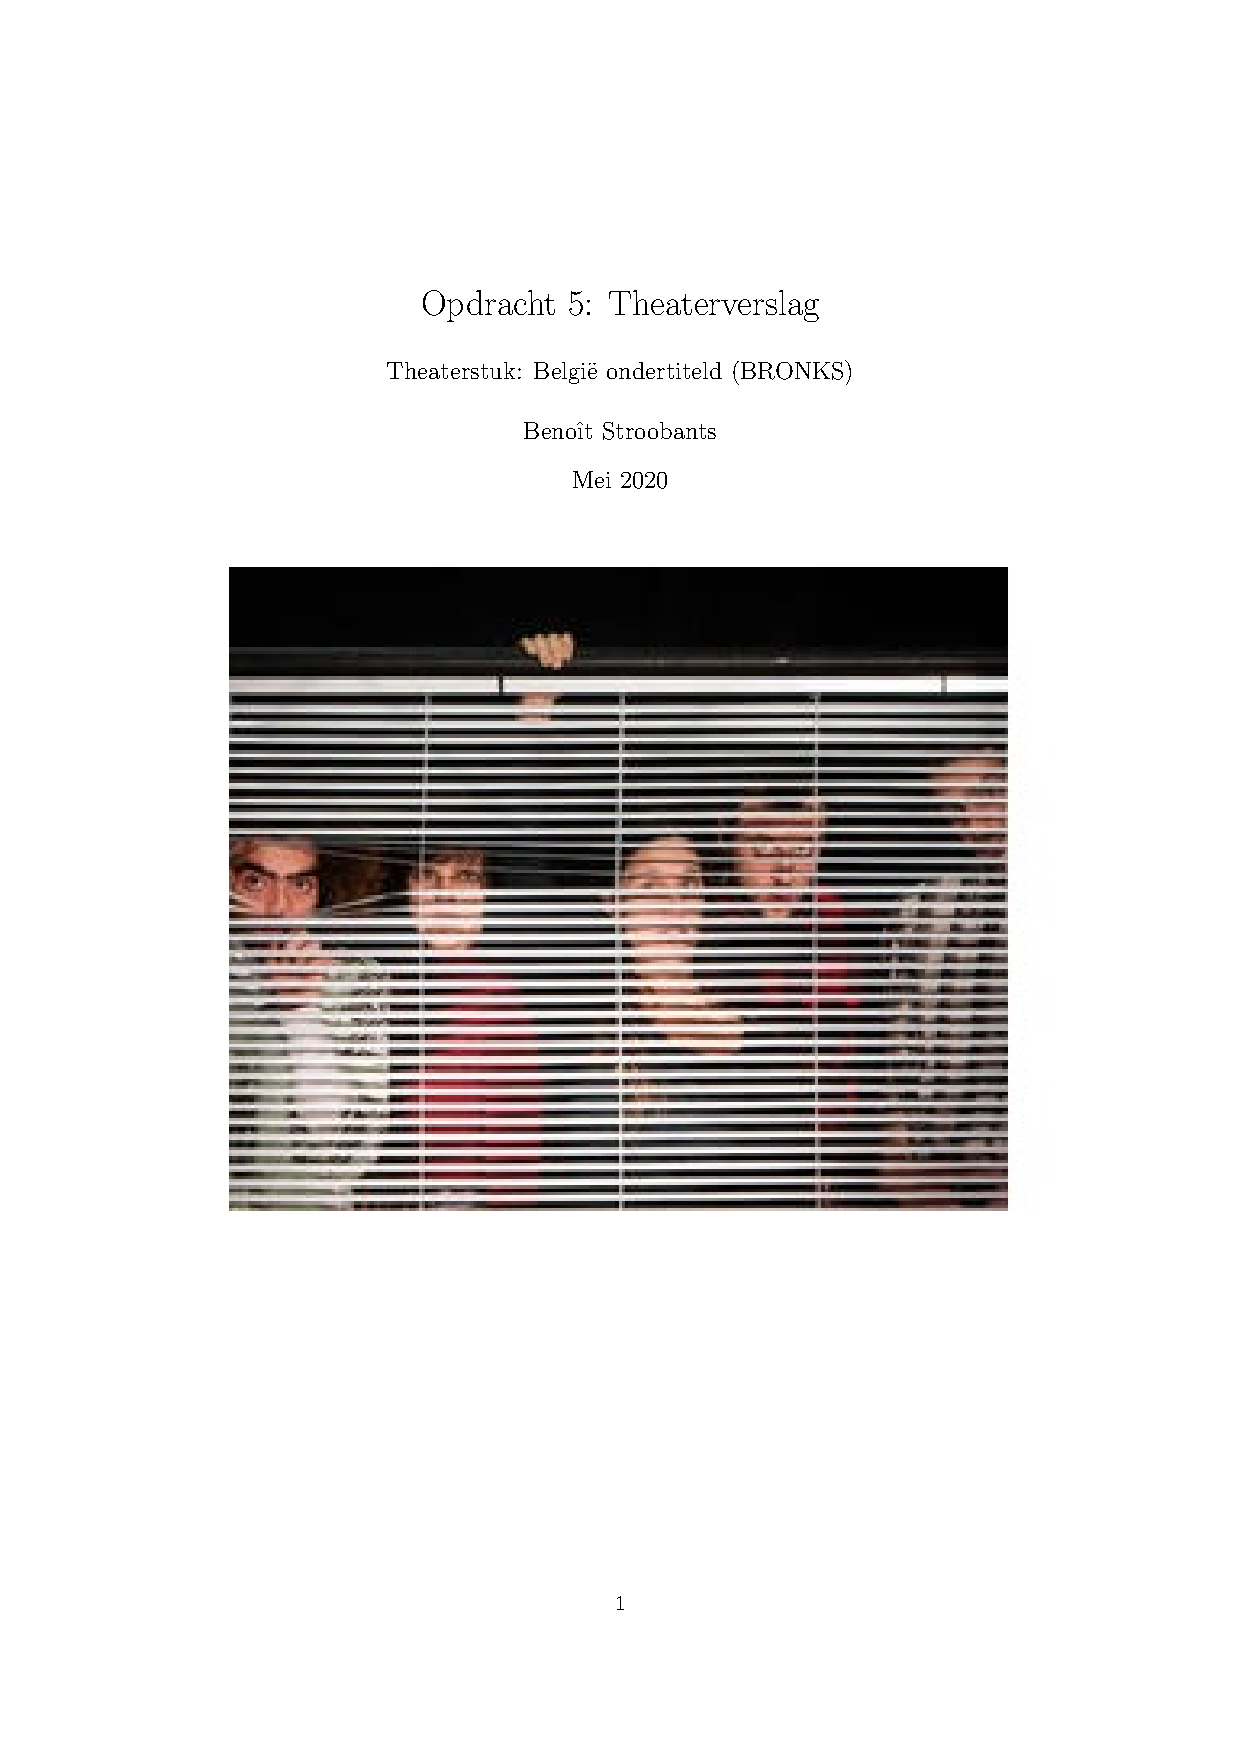
\includepdf[page=-]{Opdracht 5.pdf}

\newpage
\vspace*{\fill}
\begin{center}
\addcontentsline{toc}{section}{Opdracht 6: Een balansverslag}
\newcommand{\HRule}{\rule{\linewidth}{0.5mm}}
\HRule \\[0.4cm]
\section*{Opdracht 6: Een balansverslag}
\HRule \\[1.5cm]
\end{center}
\vspace*{\fill}
   
%\includepdf[page=-]{Opdracht 6.pdf}

\newpage


\printbibliography[heading=bibintoc,title={Bibliografie}] %Prints the entire bibliography with the titel "Whole bibliography"
         
\end{document} to your LaTeX file where you want your
% title page.
%
%%%%%%%%%%%%%%%%%%%%%%%%%%%%%%%%%%%%%%%%%
%\title{Title page with logo}
%----------------------------------------------------------------------------------------
%	PACKAGES AND OTHER DOCUMENT CONFIGURATIONS
%----------------------------------------------------------------------------------------

\documentclass[12pt]{article}
\usepackage[english]{babel}
%\usepackage[utf8x]{inputenc}
\usepackage[utf8]{inputenc}
\usepackage{amsmath}
\usepackage{graphicx}
\usepackage[colorinlistoftodos]{todonotes}
\usepackage{pdfpages}
\usepackage[
backend=biber,
style=numeric,
sorting=none
]{biblatex}

\addbibresource{sample.bib} %Imports bibliography file

\title{Bibliography management: \texttt{biblatex} package}
\author{Share\LaTeX}
\date{ }


\begin{document}

\begin{titlepage}

\newcommand{\HRule}{\rule{\linewidth}{0.5mm}} % Defines a new command for the horizontal lines, change thickness here

\center % Center everything on the page
 
%----------------------------------------------------------------------------------------
%	HEADING SECTIONS
%----------------------------------------------------------------------------------------

\textsc{\LARGE Sint-Jan-Berchmanscollege Brussel}\\[1.5cm] % Name of your university/college
\textsc{\Large Economie Wiskunde 6}\\[0.5cm] % Major heading such as course name
\textsc{\large Nederlands}\\[0.5cm] % Minor heading such as course title

%----------------------------------------------------------------------------------------
%	TITLE SECTION
%----------------------------------------------------------------------------------------

\HRule \\[0.4cm]
{ \huge \bfseries Leesportfolio}\\[0.4cm] % Title of your document
\HRule \\[1.5cm]
 
%----------------------------------------------------------------------------------------
%	AUTHOR SECTION
%----------------------------------------------------------------------------------------

\begin{minipage}{0.4\textwidth}
\begin{flushleft} \large
\emph{Leerling:}\\
Benoît \textsc{Stroobants} % Your name
\end{flushleft}
\end{minipage}
~
\begin{minipage}{0.4\textwidth}
\begin{flushright} \large
\emph{Leerkracht:} \\
Mr R. \textsc{Vandeweerdt} % Supervisor's Name
\end{flushright}
\end{minipage}\\[2cm]

% If you don't want a supervisor, uncomment the two lines below and remove the section above
%\Large \emph{Author:}\\
%John \textsc{Smith}\\[3cm] % Your name

%----------------------------------------------------------------------------------------
%	DATE SECTION
%----------------------------------------------------------------------------------------

{\large \today}\\[2cm] % Date, change the \today to a set date if you want to be precise

%----------------------------------------------------------------------------------------
%	LOGO SECTION
%----------------------------------------------------------------------------------------


\includegraphics[width=0.3\textwidth]{Foto's/Sint_Jan_Berchmanscollege_logo2.png}\\ % Include a department/university logo - this will require the graphicx package

 
%----------------------------------------------------------------------------------------

\vfill % Fill the rest of the page with whitespace

\end{titlepage}


\renewcommand*\contentsname{Inhoudstafel}

\tableofcontents
\newpage
\vspace*{\fill}
\begin{center}
\addcontentsline{toc}{section}{Opdracht 1: Ervaringsverslag}
\newcommand{\HRule}{\rule{\linewidth}{0.5mm}}
\HRule \\[0.4cm]
\section*{Opdracht 1: Ervaringsverslag \cite{1}}
\HRule \\[1.5cm]
\end{center}
\vspace*{\fill}
   
\includepdf[page=-]{Opdracht 1.pdf}
       

\newpage
\vspace*{\fill}
\begin{center}
\addcontentsline{toc}{section}{Opdracht 2: Structureel-analytisch verslag van een kortverhaal}
\newcommand{\HRule}{\rule{\linewidth}{0.5mm}}
\HRule \\[0.4cm]
\section*{Opdracht 2: Structureel-analytisch verslag van een kortverhaal \cite{2}}
\HRule \\[1.5cm]
\end{center}
\vspace*{\fill}
   
%\includepdf[page=-]{Opdracht 2.pdf}

\newpage
\vspace*{\fill}
\begin{center}
\addcontentsline{toc}{section}{Opdracht 3: Creatieve opdracht}
\newcommand{\HRule}{\rule{\linewidth}{0.5mm}}
\HRule \\[0.4cm]
\section*{Opdracht 3: Creatieve opdracht \cite{3}}
\HRule \\[1.5cm]
\end{center}
\vspace*{\fill}
   
%\includepdf[page=-]{Opdracht 3.pdf}

\newpage
\vspace*{\fill}
\begin{center}
\addcontentsline{toc}{section}{Opdracht 4: Mediagerichte opdracht}
\newcommand{\HRule}{\rule{\linewidth}{0.5mm}}
\HRule \\[0.4cm]
\section*{Opdracht 4: Mediagerichte opdracht \cite{4}}
\HRule \\[1.5cm]
\end{center}
\vspace*{\fill}
   
%
\includepdf[page=-]{Opdracht 4.pdf}

\newpage
\vspace*{\fill}
\begin{center}
\addcontentsline{toc}{section}{Opdracht 5: Een theaterverslag}
\newcommand{\HRule}{\rule{\linewidth}{0.5mm}}
\HRule \\[0.4cm]
\section*{Opdracht 5: Een theaterverslag \cite{5}}
\HRule \\[1.5cm]
\end{center}
\vspace*{\fill}
   
%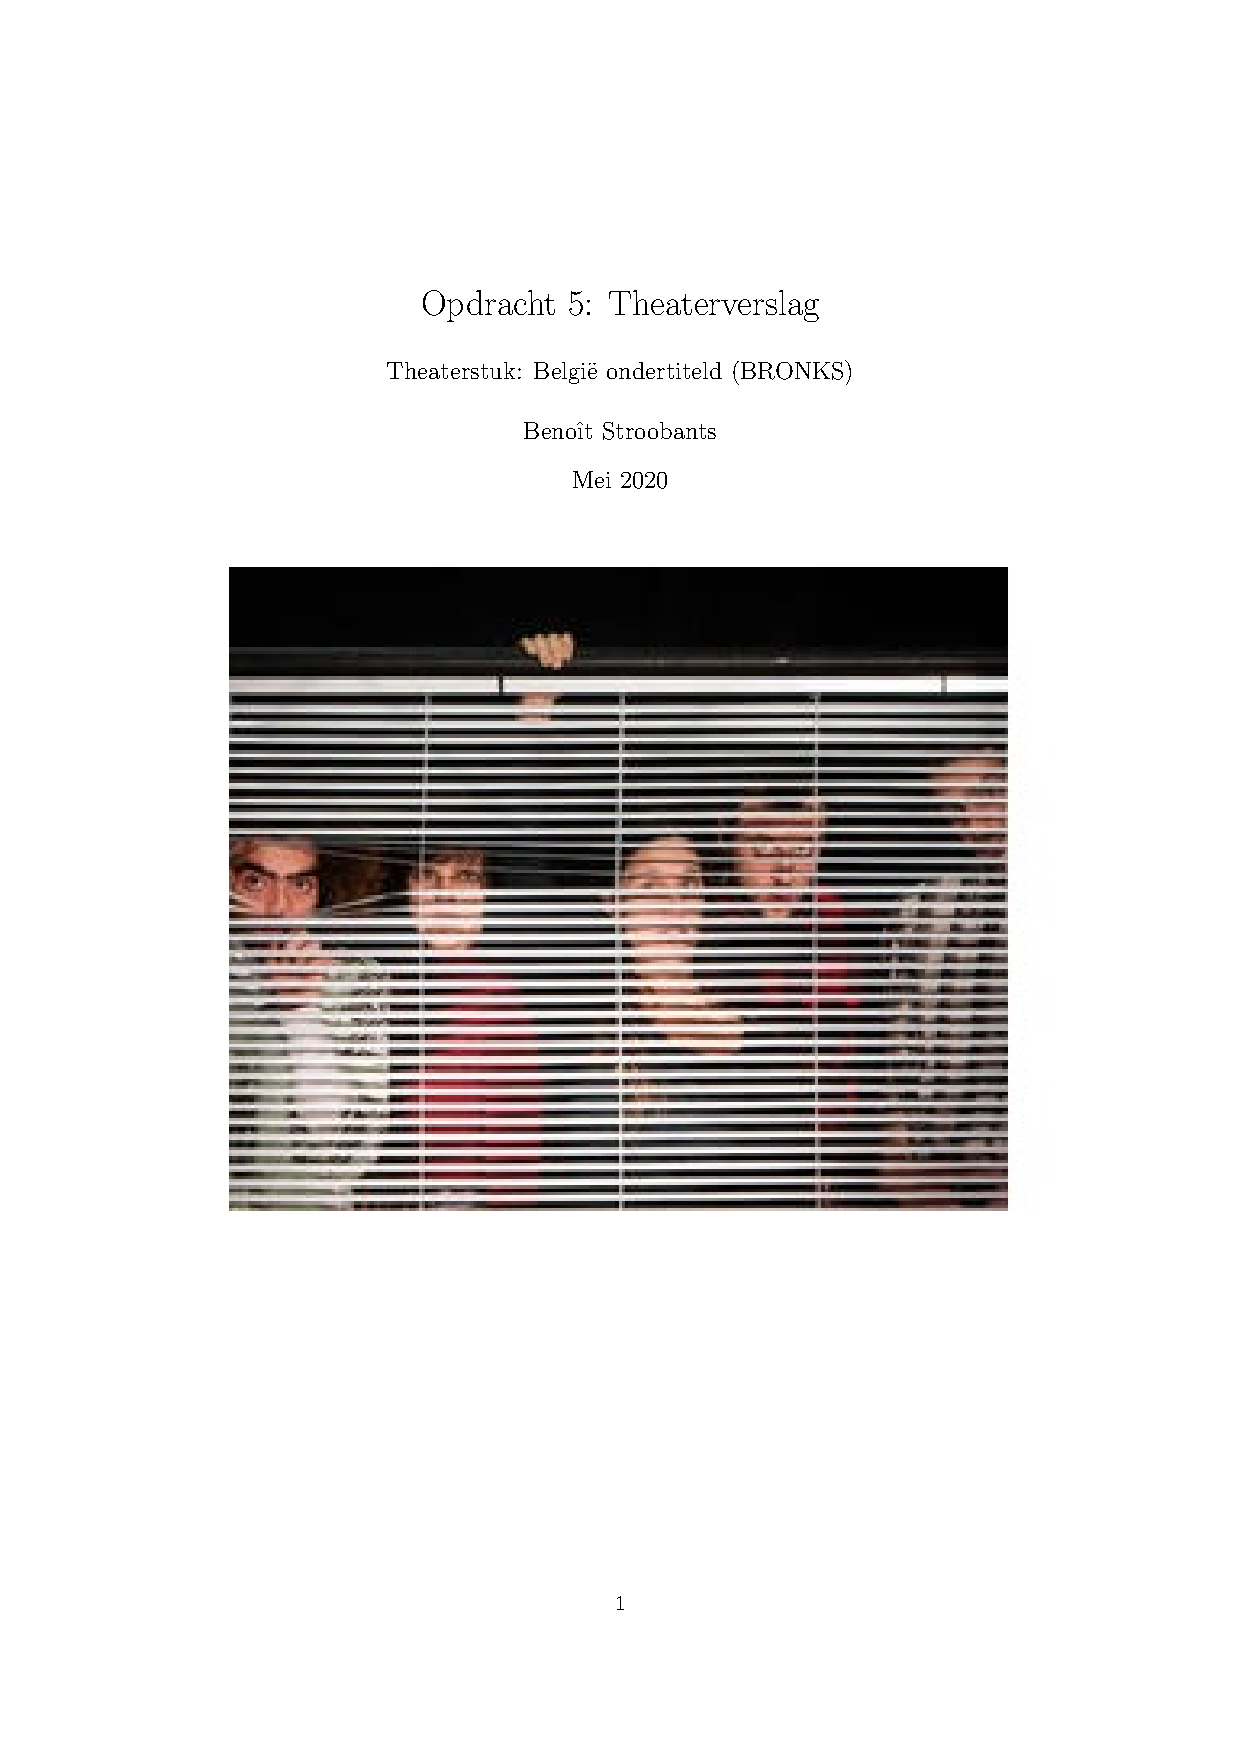
\includepdf[page=-]{Opdracht 5.pdf}

\newpage
\vspace*{\fill}
\begin{center}
\addcontentsline{toc}{section}{Opdracht 6: Een balansverslag}
\newcommand{\HRule}{\rule{\linewidth}{0.5mm}}
\HRule \\[0.4cm]
\section*{Opdracht 6: Een balansverslag}
\HRule \\[1.5cm]
\end{center}
\vspace*{\fill}
   
%\includepdf[page=-]{Opdracht 6.pdf}

\newpage


\printbibliography[heading=bibintoc,title={Bibliografie}] %Prints the entire bibliography with the titel "Whole bibliography"
         
\end{document} to your LaTeX file where you want your
% title page.
%
%%%%%%%%%%%%%%%%%%%%%%%%%%%%%%%%%%%%%%%%%
%\title{Title page with logo}
%----------------------------------------------------------------------------------------
%	PACKAGES AND OTHER DOCUMENT CONFIGURATIONS
%----------------------------------------------------------------------------------------

\documentclass[12pt]{article}
\usepackage[english]{babel}
%\usepackage[utf8x]{inputenc}
\usepackage[utf8]{inputenc}
\usepackage{amsmath}
\usepackage{graphicx}
\usepackage[colorinlistoftodos]{todonotes}
\usepackage{pdfpages}
\usepackage[
backend=biber,
style=numeric,
sorting=none
]{biblatex}

\addbibresource{sample.bib} %Imports bibliography file

\title{Bibliography management: \texttt{biblatex} package}
\author{Share\LaTeX}
\date{ }


\begin{document}

\begin{titlepage}

\newcommand{\HRule}{\rule{\linewidth}{0.5mm}} % Defines a new command for the horizontal lines, change thickness here

\center % Center everything on the page
 
%----------------------------------------------------------------------------------------
%	HEADING SECTIONS
%----------------------------------------------------------------------------------------

\textsc{\LARGE Sint-Jan-Berchmanscollege Brussel}\\[1.5cm] % Name of your university/college
\textsc{\Large Economie Wiskunde 6}\\[0.5cm] % Major heading such as course name
\textsc{\large Nederlands}\\[0.5cm] % Minor heading such as course title

%----------------------------------------------------------------------------------------
%	TITLE SECTION
%----------------------------------------------------------------------------------------

\HRule \\[0.4cm]
{ \huge \bfseries Leesportfolio}\\[0.4cm] % Title of your document
\HRule \\[1.5cm]
 
%----------------------------------------------------------------------------------------
%	AUTHOR SECTION
%----------------------------------------------------------------------------------------

\begin{minipage}{0.4\textwidth}
\begin{flushleft} \large
\emph{Leerling:}\\
Benoît \textsc{Stroobants} % Your name
\end{flushleft}
\end{minipage}
~
\begin{minipage}{0.4\textwidth}
\begin{flushright} \large
\emph{Leerkracht:} \\
Mr R. \textsc{Vandeweerdt} % Supervisor's Name
\end{flushright}
\end{minipage}\\[2cm]

% If you don't want a supervisor, uncomment the two lines below and remove the section above
%\Large \emph{Author:}\\
%John \textsc{Smith}\\[3cm] % Your name

%----------------------------------------------------------------------------------------
%	DATE SECTION
%----------------------------------------------------------------------------------------

{\large \today}\\[2cm] % Date, change the \today to a set date if you want to be precise

%----------------------------------------------------------------------------------------
%	LOGO SECTION
%----------------------------------------------------------------------------------------


\includegraphics[width=0.3\textwidth]{Foto's/Sint_Jan_Berchmanscollege_logo2.png}\\ % Include a department/university logo - this will require the graphicx package

 
%----------------------------------------------------------------------------------------

\vfill % Fill the rest of the page with whitespace

\end{titlepage}


\renewcommand*\contentsname{Inhoudstafel}

\tableofcontents
\newpage
\vspace*{\fill}
\begin{center}
\addcontentsline{toc}{section}{Opdracht 1: Ervaringsverslag}
\newcommand{\HRule}{\rule{\linewidth}{0.5mm}}
\HRule \\[0.4cm]
\section*{Opdracht 1: Ervaringsverslag \cite{1}}
\HRule \\[1.5cm]
\end{center}
\vspace*{\fill}
   
\includepdf[page=-]{Opdracht 1.pdf}
       

\newpage
\vspace*{\fill}
\begin{center}
\addcontentsline{toc}{section}{Opdracht 2: Structureel-analytisch verslag van een kortverhaal}
\newcommand{\HRule}{\rule{\linewidth}{0.5mm}}
\HRule \\[0.4cm]
\section*{Opdracht 2: Structureel-analytisch verslag van een kortverhaal \cite{2}}
\HRule \\[1.5cm]
\end{center}
\vspace*{\fill}
   
%\includepdf[page=-]{Opdracht 2.pdf}

\newpage
\vspace*{\fill}
\begin{center}
\addcontentsline{toc}{section}{Opdracht 3: Creatieve opdracht}
\newcommand{\HRule}{\rule{\linewidth}{0.5mm}}
\HRule \\[0.4cm]
\section*{Opdracht 3: Creatieve opdracht \cite{3}}
\HRule \\[1.5cm]
\end{center}
\vspace*{\fill}
   
%\includepdf[page=-]{Opdracht 3.pdf}

\newpage
\vspace*{\fill}
\begin{center}
\addcontentsline{toc}{section}{Opdracht 4: Mediagerichte opdracht}
\newcommand{\HRule}{\rule{\linewidth}{0.5mm}}
\HRule \\[0.4cm]
\section*{Opdracht 4: Mediagerichte opdracht \cite{4}}
\HRule \\[1.5cm]
\end{center}
\vspace*{\fill}
   
%
\includepdf[page=-]{Opdracht 4.pdf}

\newpage
\vspace*{\fill}
\begin{center}
\addcontentsline{toc}{section}{Opdracht 5: Een theaterverslag}
\newcommand{\HRule}{\rule{\linewidth}{0.5mm}}
\HRule \\[0.4cm]
\section*{Opdracht 5: Een theaterverslag \cite{5}}
\HRule \\[1.5cm]
\end{center}
\vspace*{\fill}
   
%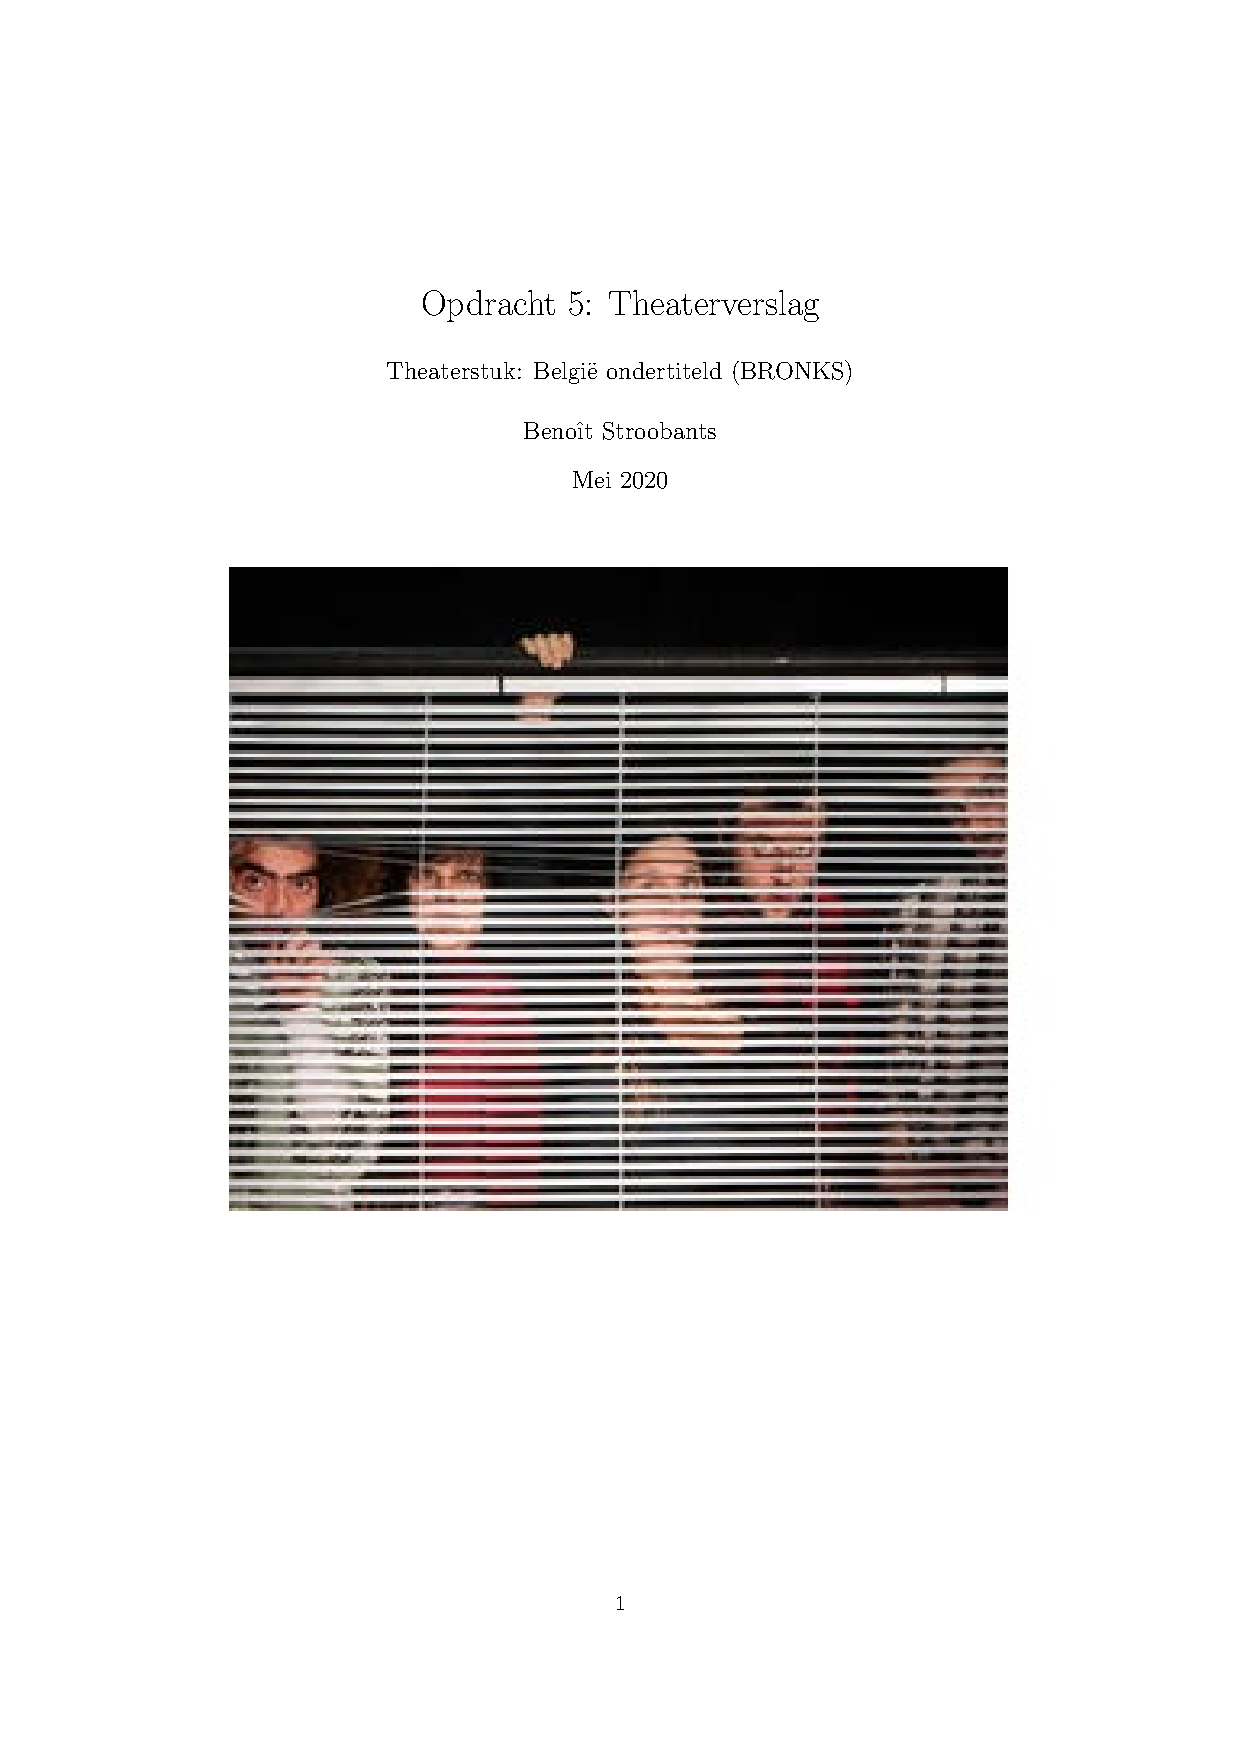
\includepdf[page=-]{Opdracht 5.pdf}

\newpage
\vspace*{\fill}
\begin{center}
\addcontentsline{toc}{section}{Opdracht 6: Een balansverslag}
\newcommand{\HRule}{\rule{\linewidth}{0.5mm}}
\HRule \\[0.4cm]
\section*{Opdracht 6: Een balansverslag}
\HRule \\[1.5cm]
\end{center}
\vspace*{\fill}
   
%\includepdf[page=-]{Opdracht 6.pdf}

\newpage


\printbibliography[heading=bibintoc,title={Bibliografie}] %Prints the entire bibliography with the titel "Whole bibliography"
         
\end{document}